\section{Results}

Individual frame results are best showcased by \cite{withCompensation}, with the threshold voltage being
set to a constant value, and the logarithmic response presented on an exponential scale:

\begin{figure}[H]
    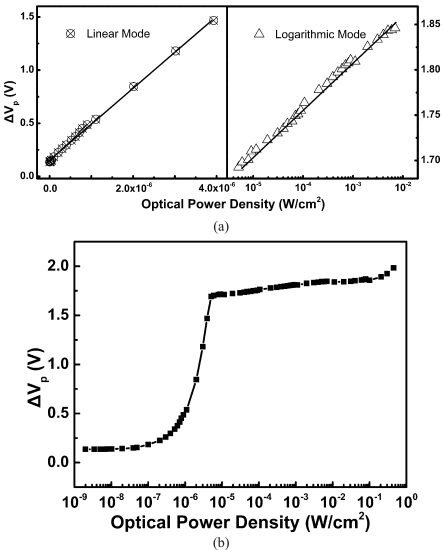
\includegraphics[width=0.50\textwidth, height=0.75\textwidth]{resources/png/response.png}
    \caption{Linear-Logarithmic response scaled. \cite{withCompensation} \label{figResponse}}
\end{figure}

As showcased in \ref{figResponse}, the output in logarithmic domain is generally greater than the reference
voltage, ensuring similar performances to previous systems. In lower light conditions however, the circuit
will remain in linear response mode, ensuring a denser value range and more accuracy when outputting low
intensity results.

Because even in linear mode the circuit can pick up spikes that reach above the \(1.5V\) reference, it is 
ensured that no pixel can be permanently locked in a feedback loop forcing a linear response after each 
iteration. At the same time, the sensitivity to significant in illumination can lead to temporary situations
in which the pixel is over-saturated for one frame. This will be, however, mitigated on the frame immediately
following, and the system will resume a stable state.


